\documentclass[tikz,border=8pt]{standalone}
% Shared look for every TikZ diagram. Load with \input{../../tools/tikz-style.tex}
\usepackage[T1]{fontenc}
\usepackage{lmodern}
\renewcommand{\sfdefault}{lmr}  % diagrams use the same serif as the text
\usetikzlibrary{arrows.meta, positioning, shapes.geometric, calc, fit, backgrounds}
\definecolor{cblue}{HTML}{4C78A8}
\definecolor{corange}{HTML}{F58518}
\definecolor{cgreen}{HTML}{54A24B}
\definecolor{cred}{HTML}{E45756}
\definecolor{cpurple}{HTML}{B279A2}
\definecolor{cgrey}{HTML}{6B6B6B}
\tikzset{
  every picture/.style={font=\sffamily, line width=1.2pt},
  box/.style={draw=#1, fill=#1!12, rounded corners=4pt, align=center, inner sep=7pt, minimum height=1.1cm},
  box/.default=cgrey,
  arrow/.style={-{Stealth[length=3mm]}, draw=cgrey, line width=1.4pt},
  title/.style={font=\sffamily\bfseries\Large},
  note/.style={font=\sffamily\small, text=cgrey, align=center},
}
\AtBeginDocument{\hyphenpenalty=10000 \exhyphenpenalty=10000}

\begin{document}
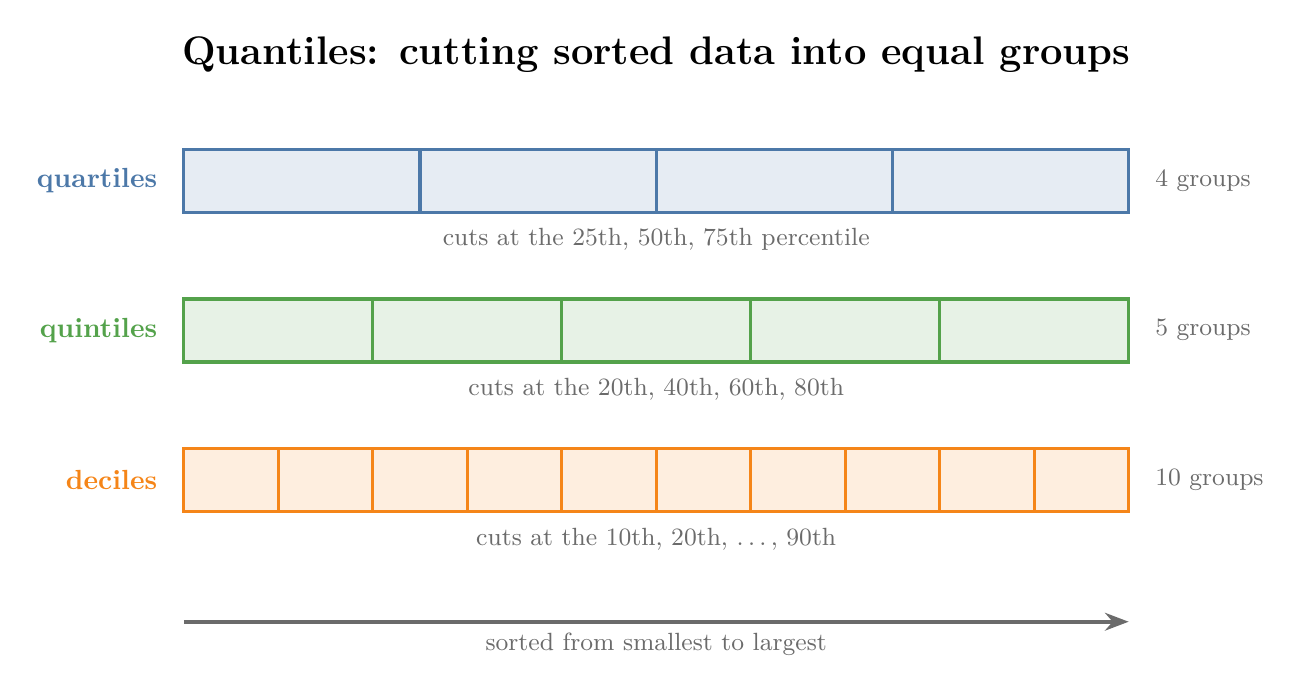
\begin{tikzpicture}[x=1cm, y=1cm]
  \node[title] at (6,1.2) {Quantiles: cutting sorted data into equal groups};
  \foreach \name/\k/\col/\y/\cuts in {quartiles/4/cblue/0/{25th, 50th, 75th percentile},
                                     quintiles/5/cgreen/-1.9/{20th, 40th, 60th, 80th},
                                     deciles/10/corange/-3.8/{10th, 20th, \dots, 90th}} {
    \foreach \i in {1,...,\k} {
      \filldraw[draw=\col, fill=\col!14] ({(\i-1)*12/\k},\y) rectangle ({\i*12/\k},\y-0.8);
    }
    \node[anchor=east, font=\sffamily\bfseries, text=\col] at (-0.2,\y-0.4) {\name};
    \node[anchor=west, font=\sffamily\small, text=cgrey] at (12.2,\y-0.4) {\k\ groups};
    \node[font=\sffamily\small, text=cgrey] at (6,\y-1.15) {cuts at the \cuts};
  }
  \draw[arrow] (0,-6.0) -- (12,-6.0) node[midway, below, font=\sffamily\small, text=cgrey] {sorted from smallest to largest};
\end{tikzpicture}
\end{document}
